\chapter{Workflows for Biodiversity Data}
\label{chapter-case-study}

In this paper we discuss two automated workflows for exchange of biodiversity data developed as part of OpenBiodiv: (1) automatic import of specimen records into manuscripts, and (2) automatic generation of data paper manuscripts from Ecological Metadata Language (EML) metadata. The workflows were presented at a webinar for the orgnization iDigBio\footnote{Integrated Digitized Biocollections (iDigBio) is a US-based aggregator of biocollections data. They hold regular webinars and workshops aimed at improving biodiversity informatics knowledge, which are attended by collection managers, scientists, and IT personnel. Thus, doing a presentation for iDigBio was an excellent way of making the research and tools-development efforts of OpenBiodiv widely known and getting feedback from the community.} and published as a paper (\cite{senderov_online_2016}).

The slides from the presentation as well as a PDF of the paper are available from the webinar GitHub page under \url{https://github.com/vsenderov/idigbio-webinar}.

\section{Abstract}

Information on occurrences of species and information on the specimens that are evidence for these occurrences (specimen records) is stored in different biodiversity databases. These databases expose the information via public REST API's. We focused on the Global Biodiversity Information Facility (GBIF), Barcode of Life Data Systems (BOLD), iDigBio, and PlutoF, and utilized their API's to import occurrence or specimen records directly into a manuscript edited in the ARPHA Writing Tool (AWT).

Furthermore, major ecological and biological databases around the world provide information about their datasets in the form of EML. A workflow was developed for creating data paper manuscripts in AWT from EML files. Such files could be downloaded, for example, from GBIF, DataONE, or the Long-Term Ecological Research Network (LTER Network).

\section{Introduction}

The webinar\footnote{Date: 16 June 2017.} presented two workflows developed as part of OpenBiodiv: (1) automatic import of occurrence or specimen records into manuscripts and (2) automatic generation of data paper manuscripts from Ecological Metadata Language (EML) metadata. The aim of the webinar was to familiarize the biodiversity community with these workflows and motivate the workflows from a scientific standpoint. The title of the webinar was "Online direct import of specimen records from iDigBio infrastructure into taxonomic manuscripts."

The development of these workflows focuses on two areas: optimizing the workflow of specimen data and optimizing the workflow of dataset metadata. These efforts resulted in the functionality that it is now possible, via a record identifier, to directly import specimen record information from the Global Biodiversity Information Facility (GBIF), Barcode of Life Data Systems (BOLD), iDigBio, or PlutoF into manuscripts in the ARPHA Writing Tool (AWT). No manual copying or retyping is required. Moreover, we created a second, data paper-based workflow.

The concept of data papers as an important means for data mobilization was introduced to biodiversity science by \cite{chavan_data_2011}. The data paper is a scholarly journal publication whose primary purpose is to describe a dataset or a group of datasets, rather than report a research investigation. Data papers serve to increase visibility, provide peer review, permanent scientific record, and credit and citation capabilities (via DOI) for biodiversity data. Thus, data papers support the effort for data to become a first class research product, and are a step forward in the direction of open science (\cite{chavan_data_2011,chavan_cultural_2013}).

Using this workflow, it is now possible to generate a data paper manuscript in AWT from a file formatted in recent EML versions.

\section{Presentation}

A video recording of the presentation is available\footnote{\url{http://idigbio.adobeconnect.com/p7sg0aym3e3/}}. More information can be found in the webinar information page\footnote{\url{http://www.idigbio.org/content/online-direct-import-specimen-records-idigbio-infrastructure-taxonomic-manuscripts}}. The slides of the presentation are attached as supplementary files and are deposited in Slideshare\footnote{\url{http://www.slideshare.net/ViktorSenderov/online-direct-import-of-specimen-records-from-idigbio-infrastructure-into-taxonomic-manuscripts}}.

During the presentation we conducted a poll about the occupation of the attendees, the results of which are summarized in Fig.~\ref{fig:webinar-poll}. Of the participants who voted, about a half were scientists, mostly biologists, while the remainder were distributed across IT specialists and librarians, with 20\% "Other." The other categories might have been administrators, decision-makers, non-biology scientists, collections personnel, educators, etc.

\begin{figure}
\centering
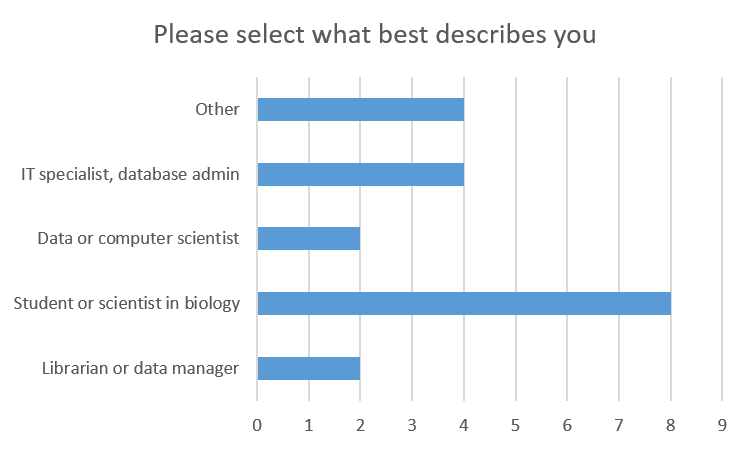
\includegraphics[width=\textwidth]{Figures/webinar-pool}
\decoRule
\caption{Poll results about composition of audience during live participation..}
\label{fig:webinar-poll}
\end{figure}

At the end of the presentation, very interesting questions were raised and discussed. For details, see the ``Results and discussion'' section of this paper.

Larry Page, Project Director at iDigBio, wrote: ``This workflow has the potential to be a huge step forward in documenting use of collections data and enabling iDigBio and other aggregators to report that information back to the institutions providing the data.''

Neil Cobb, a research professor at the Department of Biological Sciences at the Northern Arizona University, suggested that the methods, workflows and tools addressed during the presentation could provide a basis for a virtual student course in biodiversity informatics.

\section{Methods}

Both workflows discussed  rely on three key standards: RESTful API's for the web (\cite{kurtz_what_2013}), Darwin Core (\cite{wieczorek_darwin_2012}), and EML (\cite{fegraus_maximizing_2005}).

RESTful is a software architecture style for the Web, derived from the dissertation of \cite{fielding_architectural_2000}. It is out of the scope of this paper to fully explain what a RESTful API is, but a short summary follows (after \cite{kurtz_what_2013}):

\begin{itemize}
\item{URI's have to be provided for different resources.}
\item{HTTP verbs have to be used for different actions.}
\item{HATEOAS (Hypermedia as the Engine of Application State) must be implemented. This is a way of saying that the client only needs to have a basic knowledge of hypermedia, in order to use the service.}
\end{itemize}

On the other hand, Darwin Core (DwC) is a standard developed by the Biodiversity Information Standards (TDWG), also known as the Taxonomic Databases Working Group, to facilitate storage and exchange of biodiversity and biodiversity-related information. ARPHA and BDJ use the DwC terms to store taxonomic material citation data.

Finally, EML is an XML-based open-source metadata format developed by the community and the National Center for Ecological Analysis and Synthesis (NCEAS) and the Long Term Ecological Research Network (LTER, \cite{fegraus_maximizing_2005}).

\subsection{Development of workflow 1: Automated specimen record import}

There is some confusion about the terms occurrence record, specimen record, and material citation. A DwC Occurrence\footnote{\url{http://rs.tdwg.org/dwc/terms/\#Occurrence}} is defined as ``an existence of an Organism\footnote{\url{http://rs.tdwg.org/dwc/terms/\#Organism}} at a particular place at a particular time.'' The term specimen record is a term that we use for cataloged specimens in a collection that are evidence for the occurrence. In DwC, the notion of a specimen is covered by MaterialSample\footnote{\url{http://rs.tdwg.org/dwc/terms/\#MaterialSample}}, LivingSpecimen\footnote{\url{http://rs.tdwg.org/dwc/terms/\#LivingSpecimen}}, PreservedSpecimen\footnote{\url{http://rs.tdwg.org/dwc/terms/\#PreservedSpecimen}}, and FossilSpecimen\footnote{\url{http://rs.tdwg.org/dwc/terms/\#FossilSpecimen}}. The description of MaterialSample reads: "a physical result of a sampling (or sub-sampling) event. In biological collections, the material sample is typically collected, and either preserved or destructively processed." While there is a semantic difference between an occurrence record (DwC Occurrence) and a specimen record (DwC MaterialSample, LivingSpecimen, PreservedSpecimen, or FossilSpecimen), from the view point of pure syntax, they can be considered equivalent since both types of objects\footnote{We are using the term objects here in the computer science sense of the word to denote generalized data structures.} are described by the same fields in our system grouped in the following major groups:

\begin{itemize}
\item{Record-level information}
\item{Event}
\item{Identification}
\item{Location}
\item{Taxon}
\item{Occurrence}
\item{Geological context}
\end{itemize}

Taxonomic practice dictates that authors cite the materials their analysis is based on in the treatment section of the taxonomic paper (\cite{catapano_taxpub:_2010}). Therefore, in our system, as it is a document-authoring system, we take the view that these objects are material citations, i.e. bibliographic records that refer to a particular observation in the wild or a specimen in a museum. As a Supplementary material 1\footnote{The supplementary files as well as the article itself can be found under \url{https://github.com/vsenderov/idigbio-webinar}.} to the iDigBio article (\cite{senderov_online_2016}), we have attached a spreadsheet listing all DwC terms describing a specimen or occurrence record that can be imported into AWT as a material citation. From here on, we will refer to the objects being imported as specimen records, and to the objects that are part of the manuscript as material citations.

At the time when development of the workflow started, AWT already allowed import of specimen records as material citations via manual interface and via spreadsheet (Suppl. material 1 of \cite{senderov_online_2016}). So, the starting point for the development of the workflow was to locate API's for downloading biodiversity and biodiversity-related data from major biodiversity data providers and to transform the data that was provided by these API's into DwC-compatible data, which was then to be imported into the manuscript. We chose to work with GBIF, BOLD Systems, iDigBio and the PlutoF platform.

In Suppl. material 2 of \cite{senderov_online_2016} we give all the necessary information about the API's and how to map their results to DwC: endpoints, documentation, and the mapping of terms. GBIF and iDigBio name their fields in accordance with DwC, whereas for PlutoF and BOLD Systems there is a direct mapping given in the spreadsheet.

In order to abstract and reuse source code we have created a general Occurrence class, which contains the code that is shared between all occurrences, and children classes GbifOccurrence, BoldOccurrence, IDigBioOccurrence, and PlutoFOccurrence, which contain the provider-specific code. The source code is written in PHP.

\subsection{Development of workflow 2: Automated data paper generation}

Data papers are scholarly articles describing a dataset or a data package (\cite{chavan_data_2011}). Similarly, metadata are data about a dataset (\cite{michener_meta-information_2006}). Ecological metadata can be expressed in an XML-language called EML (\cite{fegraus_maximizing_2005}). It formalizes the set of concepts needed for describing ecological data (\cite{fegraus_maximizing_2005}). It is broad enough and allows dataset authors from neighboring disciplines (e.g. taxonomy) to annotate their datasets with it. We asked ourselves the question: would it be possible to convert such metadata into a data paper manuscript? As the data paper manuscript in AWT is also stored as XML (for format details see the Pensoft API\footnote{Pensoft API available under \url{http://arpha.pensoft.net/dev/}.}), all that was needed was an XSLT transformation mapping the fields of EML to the fields in the data paper XML. We have created two such transformations, for EML version 2.1.1 and for EML version 2.1.0, which we've attached as Suppl. material 3. The workflow has been tested with EML metadata downloaded from GBIF, DataONE and the LTER Network, however, it can be used for EML metadata from any other data provider.

\section{Results and Discussion}

\subsection{Workflow 1: Automated specimen record import into manuscripts developed in the ARPHA Writing Tool}

\subsubsection{Implementation}

It is now possible to directly import a specimen record as a material citation in an ARPHA Taxonomic Paper from GBIF, BOLD, iDigBio, and PlutoF (Slide 5, as well as Fig.~\ref{fig:workflow-idigbio}). The workflow from the user's perspective has been thoroughly described in a blog post; concise stepwise instructions are available via ARPHA's Tips and tricks guidelines. In a nutshell, the process works as follows:

\begin{enumerate}
\item{At one of the supported data portals (BOLD, GBIF, iDigBio, PlutoF), the author locates the specimen record he/she wants to import into the Materials section of a Taxon treatment (available in the Taxonomic Paper manuscript template).}
\item{Depending on the portal, the user finds either the occurrence identfier of the specimen, or a database record identifier of the specimen record, and copies that into the respective upload field of the ARPHA system (Fig.~\ref{fig:occurrence-input-mask}).}
\item{After the user clicks on ``Add,'' a progress bar is displayed, while the specimens are being uploaded as material citations.}
\item{The new material citations are rendered in both human- and machine-readable DwC format in the Materials section of the respective Taxon treatment and can be further edited in AWT, or downloaded from there as a CSV file.}
\end{enumerate}

\begin{figure}
\centering
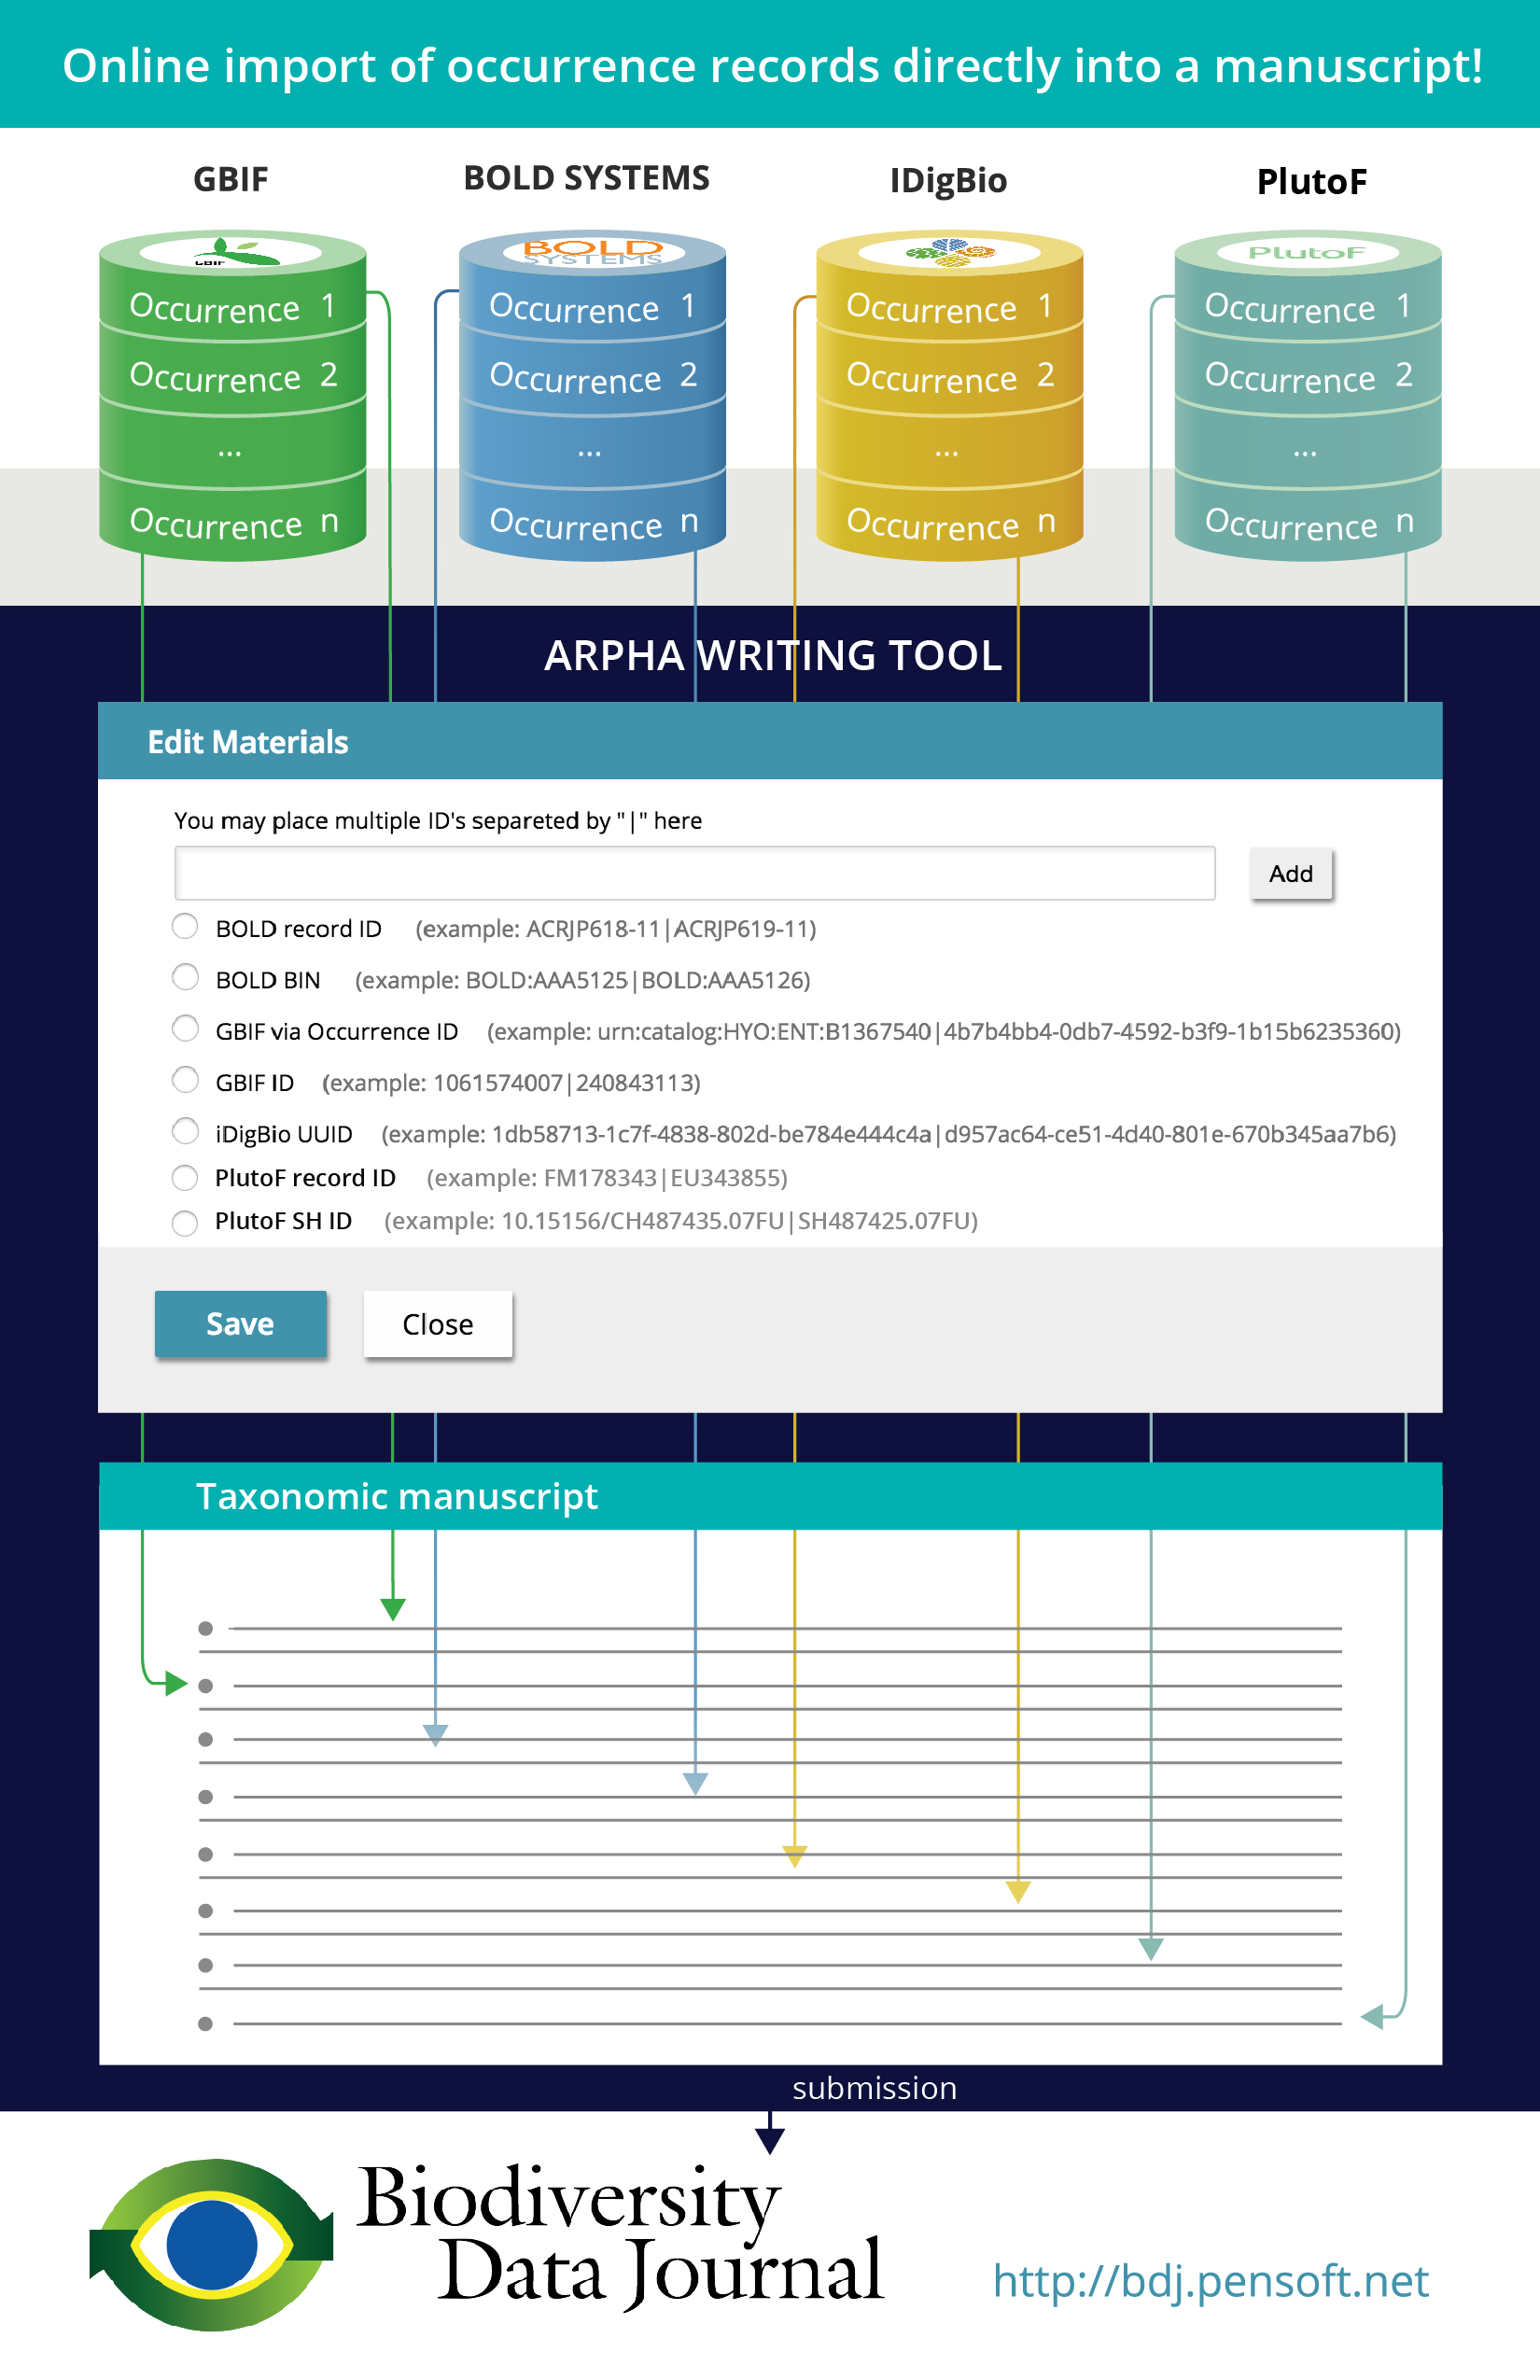
\includegraphics[width=\textwidth]{Figures/workflow-idigbio}
\decoRule
\caption{This fictionalized workflow presents the flow of information content of biodiversity specimens or biodiversity occurrences from the data portals GBIF, BOLD Systems, iDigBio, and PlutoF, through user-interface elements in AWT to textualized content in a Taxonomic Paper manuscript template intended for publication in the Biodiversity Data Journal.}
\label{fig:workflow-idigbio}
\end{figure}

\begin{figure}
\centering
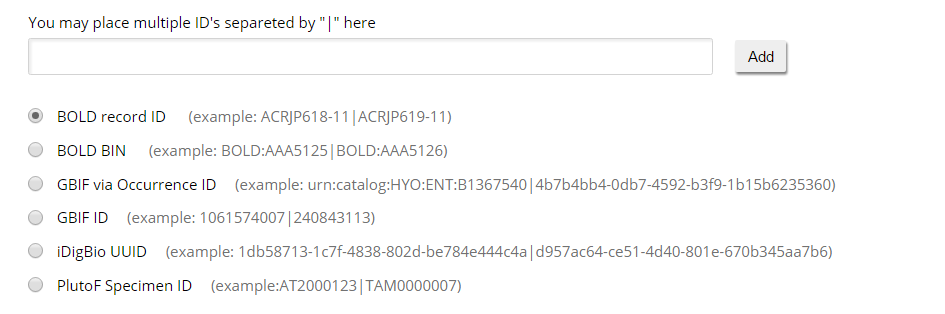
\includegraphics[width=\textwidth]{Figures/occurrence-input-mask}
\decoRule
\caption{User interface of the ARPHA Writing Tool controlling the import of specimen records from external databases.}
\label{fig:occurrence-input-mask}
\end{figure}

\paragraph{Discussion.} The persistent unique identifiers (PID's) are a long-discussed problem in biodiversity informatics (\cite{guralnick_trouble_2014}). Questions of fundamental importance are: given a specimen in a museum, is it (and how often is it) cited in a paper? What about the quality of the database record belonging to this specimen? In order for us to be able to answer these questions to our satisfaction, specimens need to have their own unique identifiers, which are imported as part of the material citation and allow the researcher to scan through the body of published literature to find which specimens have been cited (and how often). In practice, however, this is not always the case and we have to rely on the DwC triplet, ({\tt institutionCode}, {\tt collectionCode}, {\tt catalogNumber}), to positively identify specimens (\cite{guralnick_trouble_2014}). In the next paragraphs, we discuss how the information provided by the repositories can be used to track material citations.

\paragraph{GBIF.} Import from GBIF is possible both via a DwC {\tt occurrenceID}, which is the unique identifier for the specimen/ occurrence, or via a GBIF ID, which is the record ID in GBIF's database. Thanks to its full compliance with DwC, it should be possible to track specimens imported from GBIF.

\paragraph{BOLD Systems.} In the BOLD database, specimen records are assigned an identifier, which can look like {\tt ACRJP619-11}. This identifier is the database identifier and is used for the import; it is not the identifier issued to the specimen stored in a given collection. However, some collection identifiers are returned by the API call and are stored in the material citation, for example, DwC catalogNumber and DwC institutionCode (see mappings in Suppl. material 2 in \cite{senderov_online_2016}). In this case, we have what is called a DwC doublet (\cite{guralnick_trouble_2014}), which provides us with the minimum amount of information to attempt an identification.

A feature of BOLD Systems is that records are grouped into BIN's representing Operational Taxonomic Units (OTU's) based on a hierarchical/ graph-based clustering algorithm (\cite{ratnasingham_dna-based_2013}). It is possible to import all specimen records from a BIN in a single step, specifying the BIN ID. This streamlines the description of new species from OTU's as it allows the taxonomist to save time and import all materials from the BIN.

\paragraph{iDigBio.} iDigBio provides its specimen records in a DwC-compatible format. Similar to GBIF, both a DwC occurrenceID, as well as DwC triplet information is returned by the system and stored in our XML making tracking of specimen citations easy.

\paragraph{PlutoF.} Import from PlutoF is attained through the usage of a specimen ID (DwC catalogNumber), which is disambiguated to a PlutoF record ID by our system. If a specimen ID matches more than one record in the PlutoF system, multiple records are imported and the user has to delete the superfluous material citations. PlutoF does store a full DwC triplet while no DwC occurrenceID is available for the time being.

Ultimately, this workflow can serve as a curation filter for increasing the quality of specimen data via the scientific peer review process. By importing a specimen record via our workflow, the author of the paper vouches for the quality of the particular specimen record that he or she presumably has already checked against the physical specimen. Then a specimen that has been cited in an article can be marked with a star as a peer-reviewed specimen by the collection manager. Also, the completeness and correctness of the specimen record itself can be improved by comparing the material citation with the database record and synchronizing differing fields.

There is only one component currently missing from for this curation workflow: a query page that accepts a DwC occurrenceID or a DwC doublet/ triplet and returns all the information stored in the Pensoft database regarding material citations of this specimen.

\subsection{Workflow 2: Automated data paper manuscript generation from EML metadata in the ARPHA Writing Tool}

\paragraph{Implementation.} We have created a workflow that allows authors to automatically create data paper manuscripts from the metadata stored in EML. The completeness of the manuscript created in such a way depends on the quality of the metadata; however, after generating such a manuscript, the authors can update, edit, and revise it as any other scientific manuscript in the AWT. The workflow has been thoroughly described in a blog post; concise stepwise instructions are available via ARPHA's Tips and tricks guidelines. In a nutshell, the process works as follows:

\begin{enumerate}
\item{The users of ARPHA need to save a dataset's metadata as an EML file (versions 2.1.1 and 2.1.0, support for other versions is being continually updated) from the website of the respective data provider (see Fig.~\ref{fig:EML-download} as an example using the GBIF's Integrated Publishing Toolkit (IPT)). Some leading data portals that provide such EML files are GBIF (EML download possible both from IPT and from the portal), DataONE, and the LTER Network.}
\item{Click on the ``Start a manuscript'' button in AWT and then select ``Biodiversity Data Journal'' and the ``Data paper (Biosciences)'' template (Fig.~\ref{fig:journal-selection}).}
\item{Upload this file via the "Import a manuscript" function on the AWT interface (Fig.~\ref{fig:user-interface}).}
\item{Continue with updating and editing and finally submit your manuscript inside AWT.}
\end{enumerate}

\begin{figure}
\centering
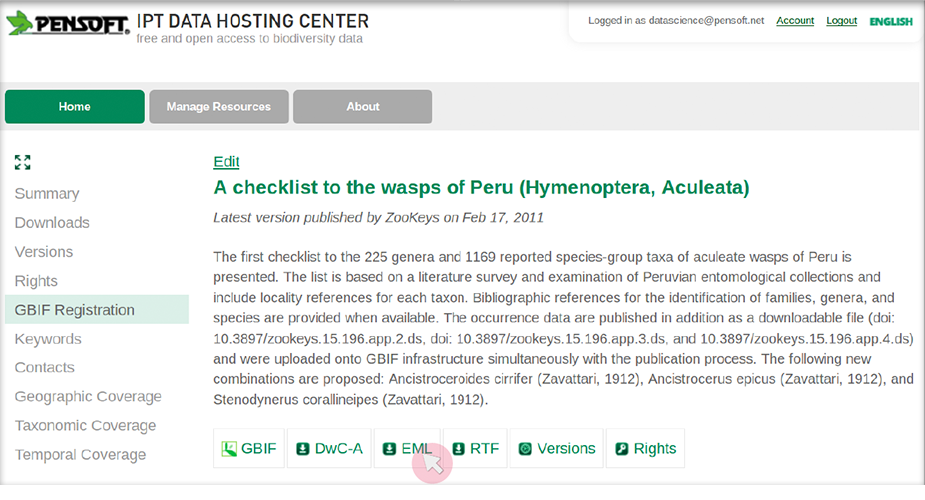
\includegraphics[width=\textwidth]{Figures/EML-download}
\decoRule
\caption{Download of an EML from the GBIF Integarted Publishuing Toolkit (IPT).}
\label{fig:EML-download}
\end{figure}

\begin{figure}
\centering
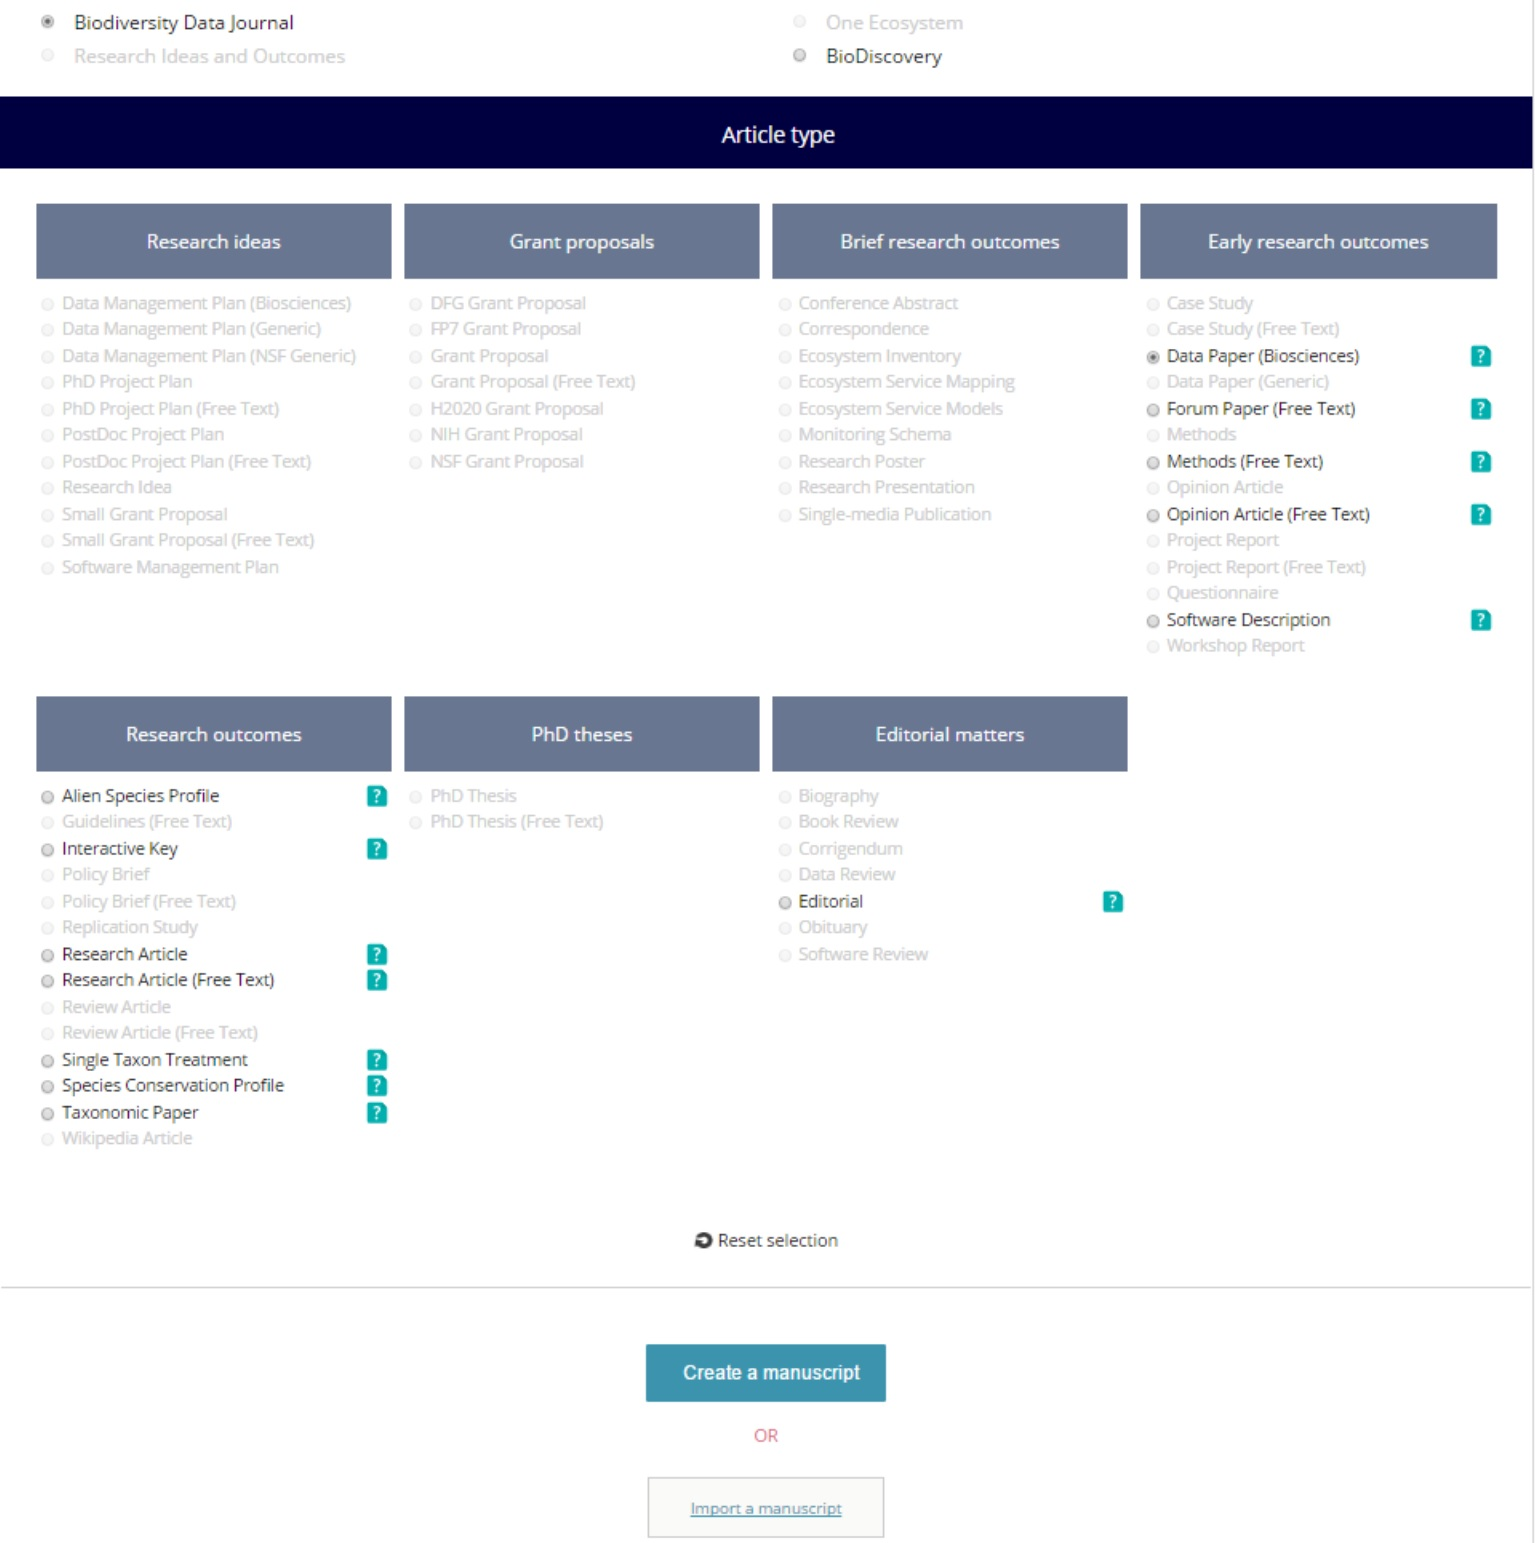
\includegraphics[width=\textwidth]{Figures/journal-selection}
\decoRule
\caption{Selection of the journal and ``Data Paper (Biosciences)'' template in the ARPHA Writing Tool.}
\label{fig:journal-selection}
\end{figure}

\begin{figure}
\centering
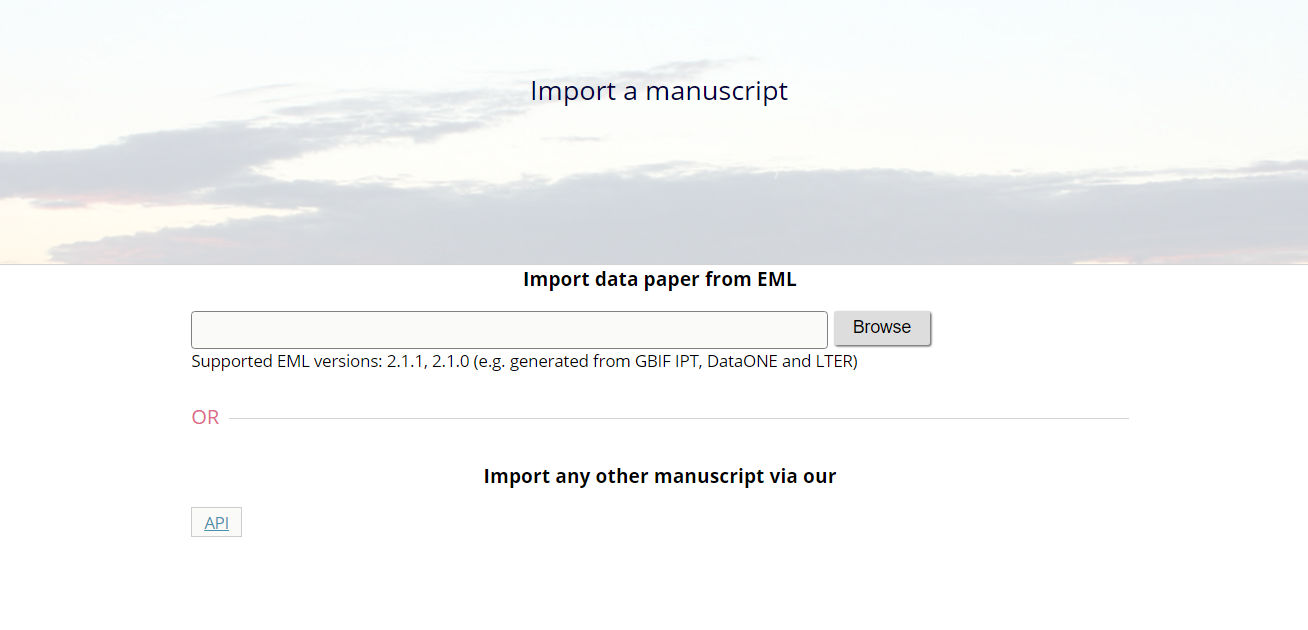
\includegraphics[width=\textwidth]{Figures/user-interface}
\decoRule
\caption{The user interface field for uploading EML files into ARPHA.}
\label{fig:user-interface}
\end{figure}

\paragraph{Discussion} In 2010, GBIF and Pensoft began investigating mainstream biodiversity data publishing in the form of ``data papers.'' As a result this partnership pioneered a workflow between GBIF’s IPT and Pensoft’s journals, viz.: ZooKeys, MycoKeys, Phytokeys, Nature Conservation, and others. The rationale behind the project was to motivate authors to create proper metadata for their datasets to enable themselves and their peers to properly make use of the data. Our workflow gives authors the opportunity to convert their extended metadata descriptions into data paper manuscripts with very little extra effort. The workflow generates data paper manuscripts from the metadata descriptions in IPT automatically at the "click of a button." Manuscripts are created in Rich Text Format (RTF) format, edited and updated by the authors, and then submitted to a journal to undergo peer review and publication. The publication itself bears the citation details of the described dataset with its own DOI or other unique identifier. Ideally, after the data paper is published and a DOI is issued for it, it should be included in the data description at the repository where the data is stored. Within less than four years, a total of more than 100 data papers have been published in Pensoft's journals (examples: \cite{brosens_formidabel:_2013}, \cite{desmet_database_2013}, \cite{gutt_antarctic_2013}, \cite{pierrat_antarctic_2012}, \cite{shao_dataset_2012}, \cite{tng_vegetation_2016}). The workflow and associated author guidelines are described in \cite{penev_pensoft_2016}.

The present chapter describes the next technological step in the generation of data papers: direct import of an EML file via an API into a manuscript being written in AWT. A great advantage of the present workflow is that data paper manuscripts can be edited and peer-reviewed collaboratively in the authoring tool even before submission to the journal. These novel features provided by AWT and BDJ may potentially become a huge step forward in experts' engagement and mobilization to publish biodiversity data in a way that facilitates recording, credit, preservation, and re-use. Another benefit of this usage of EML data might be that in the future, more people wil provide more robust EML data files.

\paragraph{Feedback.} The two workflows presented generated a lively discussion at the end of the presentation, which we summarize below:

\begin{enumerate}
\item{Are specimen records imported from GBIF and then slightly changed during the editorial process then deduplicated at GBIF? Answer: Unfortunately, no. At GBIF, deduplication only occurs for identical records.}
\item{Are we leaving the identifiers from GBIF or iDigBio in the records? Answer: Yes. We have made the best effort to import specimen record identifiers. This has been discussed in the previous sections.}
\item{How will the tool reduce the input time for constructing a manuscript? Answer: AWT reduces the time for creating a manuscript in two significant ways. First of all, the workflows avoid retyping of specimen records or metadata. Secondly, another time-saving feature is the elimination of copying errors. Creating of data paper manuscripts from EML saves, as a minimum, the effort of copy-pasting metadata and their arrangement in a manuscript.}
\item{What are the major hurdles or challenges left in having this become a mainstream tool? How mature is the tool? Answer: We believe that the main hurdles in this becoming a main-stream tool are visibility and awareness of the tool by the community, as the stability of the software is already at a very good stage.}
\item{Is it possible to track the usage of museum specimens for data aggregators? Answer: Yes, see question 2 and discussion in the present section.}
\item{How do you go to the article page where collection managers can search for data published from their collections on the Pensoft website? Answer: We are working on the streamlining of this functionality. It will be part of the OBKMS. Currently, we markup collection codes against the Global Registry of Biodiversity Repositories (GRBio\footnote{GRBio is available under \url{http://grbio.org/}}) vocabularies, and the reader can view the records from a particular collection by clicking on the collection code.}
\end{enumerate}